%!TEX root =  main.tex

\documentclass{article}

%% make sure you have the nature.cls and naturemag.bst files where
\usepackage{algorithm}
\usepackage{algorithmic}
\usepackage{amsmath,graphicx}
\usepackage{url}
\bibliographystyle{naturemag}
\usepackage{color}
\newcommand{\comment}[1]{}

\title{Computer vision profiling of neurite outgrowth morphodynamic phenotypes}

%% Notice placement of commas and superscripts and use of &
%% in the author list

%\author{Ludovico Fusco$^{1,7}$, Fethallah Benmansour$^{2, 7}$, Riwal Lefort$^{3, 7}$, Kevin Smith$^{4, 7}$, German Gonzales$^5$,  Catherina Barillari$^6$, Bernd Rinn$^6$, Pascal Fua$^2$, Francois Fleuret$^3$   \& Olivier Pertz$^1$}


%======================================================================
\begin{document}

\maketitle

In this supplementary document, we describe and evaluate the computer vision pipeline that allowed to automatically segment and track the soma and neurites in each frame of the timelapse datasets.

%Our approach first detects nuclei and associated somata at each time step. The nucleus of each neuron is detected as a Maximally Stable Extremal Region (MSER)~\cite{Nister:2008} from the Cherry channel. Using the detected nuclei as seed points, a region-growing algorithm segments the neuron�s soma. Next, the implemented multi-objects tracking algorithm~\cite{BerclazTPAMI2011} searches through the full set of nuclei and somata detections to extract the best K-shortest paths according to a similarity measure between two detections. The proposed similarity measure is derived from the Earth Mover�s Distance~\cite{Pele-iccv2009} between the intensity histograms of the detected somata regions (in the supplementary note 3, we show that this distance provides a good tradeoff between efficiency and precision).  Neurons are detected and tracked at an accuracy of (TODO 95\%) (still waiting for the GT to be completed for number crunching); �Finally, the tracked somata are used to initialize a neurite segmentation and association algorithm based on shortest path computation and Voronoi tessellation. Comparison to manually annotated data demonstrates that �(URGENT TODO: crunch the numbers: still waiting for the GT)�
%======================================================
\section{Data description and ground truth}
%======================================================
%----------------------------------------------------------------------------
\subsection{Input data description and notations}
%----------------------------------------------------------------------------
The  input to  our approach  is a  series of  $T$ images  $\mathcal{I}  = \{I_1,
\ldots,  I_t,  \ldots, I_T\}$  from  which  we  extract $K$  nucleus  detections
$d_t^k$.   The  tracking step  described  in Sec.~\ref{sec:tracking}  associates
valid detections  across time steps  while rejecting spurious  detections. Since
each neuron  contains only  one nucleus, there  is a one-to-one  mapping between
each valid  nucleus detection $c_t^i$ and  a neuron $X_t^i$.  Thus, the tracking
task   is   to  provide   a   set   of   neuron  detections   $\mathcal{X}^i   =
\{X_{a}^i,\ldots,X_t^i,\ldots,X_{b}^i \}$ defining an individual neuron $i$ from
time  $t=a$  to $t=b$.   As  depicted  in  Fig.~\ref{fig:notation}, each  neuron
detection $X_t^i$ is composed of a nucleus $c_t^i$, a soma $s_t^i$, a set of $J$
neurites $\{n_t^{i,1},  \ldots, n_t^{i,j}, \ldots,  n_t^{i,J} \}$, and a  set of
$L$     filopodia    associated     with    each     neurite     $F_t^{i,j}    =
\{f_t^{i,j,1},\ldots,f_t^{i,j,l},\ldots,f_t^{i,j,L}  \}$ so  that  $N_t^i =  \{(
n_t^{i,1},F_t^{i,1}), \ldots,(n_t^{i,j},F_t^{i,j}) \}$.  Thus, a complete neuron
$i$  at time step $t$ is described by $X_t^i = \{ c_t^i, s_t^i, N_t^i \}$.

%----------------------------------------------------------------------------
\begin{figure}[!h]
  \begin{center}
       \begin{tabular}{@{\hspace{-1mm}}c}
        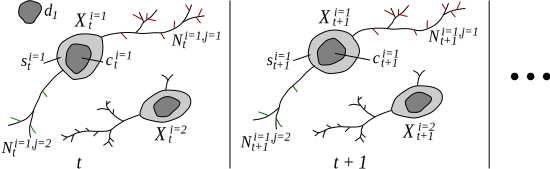
\includegraphics[width = 0.8\linewidth] {images/neurondrawing.pdf}\\ [-2.4ex]
       \end{tabular} 
    \caption{ \footnotesize   Neuron  tracking  notation.  At time $t$ a neuron $i$ detection $X_t^i = \{ c_t^i,
        s_t^i, N_t^i  \}$ contains a nucleus $c_t^i$,  a soma $s_t^i$,
        and    a  set of   neurite-filopodia    tuples    $N_t^i     =    \{(
        n_t^{i,1},F_t^{i,1}),   \ldots,(n_t^{i,j},F_t^{i,j}),  \ldots,
        (n_t^{i,J},F_t^{i,J})  \}$  which  contains $J$  neurites  and
        their associated  filopodia shown in  red for $j=1$  and green
        for  $j=2$. A spurious nucleus  detection  $d_1$ is also shown.
        A neuron $i$  is defined by  a time-series of  neuron detections
        $\mathcal{X}^i     =     \{X_{a}^i,\ldots,X_t^i,\ldots,X_{b}^i
        \}$.  The  tracking returns  a  set  $\mathcal{X}^i$ for  each
        neuron. }
    \label{fig:notation}
  \end{center}
\end{figure}
%% by linking nucleus detections  and ``growing'' the
%%         neuron from the nucleus seed
%----------------------------------------------------------------------------



%----------------------------------------------------------------------------
\subsection{Ground truth}
%----------------------------------------------------------------------------
In order to evaluate our automatic algorithm, we manually annotated cell bodies and neurites using appropriate tools as described hereinafter.
We clearly distinguished between two annotation tasks: 
\begin{itemize}
\item segmentation and tracking of nuclei and somata from dynamic sequences,
\item segmentation of neurite trees from static images.
\end{itemize}
We clearly made this distinction because we could not find an appropriate semi-automatic or manual software for tracking the neurites. Therefore, even if our automatic pipeline is able to track neurites, only the quality of neurite trees at a given time frame will we assessed.

Our computer vision pipeline have been applied to two different sets of sequences acquired using two different magnifications: \texttt{10x} and \texttt{20x}. Therefore, we made random selections from each magnification set, and conducted our evaluation on each of them independently.
 
\subsubsection{Cell body ground truth}
To manually segment and track nuclei and somata from dynamic sequences, we used \texttt{TrakEM2}\footnote{publicly available at \url{http://www.ini.uzh.ch/~acardona/trakem2.html}}, a plugin of FIJI / ImageJ. To ease the annotation step, the input sequences have been encoded in a single multipage tiff file for each channel, and an xml file have been generated for each sequence to encode the segmentation and tracking data structure (see supplemental material).
\begin{itemize}
\item 12 sequences have been randomly selected from the \texttt{20x} dataset. From these sequences, 79 cells have been tracked, representing 4709 annotated nuclei and somata.
\item 3 sequences have been randomly selected from the \texttt{10x} dataset. From these sequences, 29 cells have been tracked, representing 2152 annotated nuclei and somata.
\end{itemize}


\subsubsection{Neurite ground truth}
To segment neurite trees from static images, we used an improved version of the Simple Neurite Tracer (SNT) plugin. The SNT plugin\footnote{\url{http://fiji.sc/wiki/index.php/Simple_Neurite_Tracer}}, a FIJI plugin, is a semi-automatic tool meant to reduce user' interaction for neuronal tree tracing . Recently, an improved version of SNT have been released \url{http://cvlab.epfl.ch/software/delin/index.php}, allowing a better description of the neurite branches, including their width estimate and more accurate centeline extraction as shown in figure~\ref{fig:annotations}.

Similarly to the dynamic dataset, we randomly selected images from the two different magnification sets, and annotated all visible neurite trees:
\begin{itemize}
\item 30 images from the 20x dataset have been randomly selected. 223 neurite trees or neurite branches have been annotated.
\item 27 images from the 10x dataset have been randomly selected. 257 neurite trees or neurite branches have been annotated.
\end{itemize}

Filopodia have been annotated only on images from the 20x dataset.
%----------------------------------------------------------------------------
\begin{figure}[!t]
  \begin{center}
       \begin{tabular}{@{\hspace{1mm}}c@{\hspace{1mm}}c}
        \includegraphics[width = 0.5\textwidth] {images/TrakEM2_Example.png} & \includegraphics[width = 0.5\textwidth] {images/TrakEM2_Example2.png}\\
                \includegraphics[width = 0.5\textwidth] {images/SNT_015_Or.png} & \includegraphics[width = 0.5\textwidth] {images/SNT_015_Seg.png}\\ 
       \end{tabular} 
    \caption{ \footnotesize  Ground truth annotation. First row, neuron tracking annotation using the \texttt{TrakEM2} plugin. Two different time frames are displayed. 
    Second row, Neurite trees annotation using the Simple Neurite Tracer plugin. On the left, the original image, and on the right the manual annotation overlaid on the image.}
    \label{fig:annotations}
  \end{center}
\end{figure}
%----------------------------------------------------------------------------


%======================================================
\section{Nuclei and somata segmentation}\label{sec:nuc}
%======================================================
\subsection{Nuclei Detection}
The  first  step in  our  approach  is to  extract  a  set of  nucleus
detections $\{d^1,\ldots,d^K\}$ over the  image series. We worked with
two-channel  images where the  cytoskeleton  is marked  with Lifeact-GFP and  nuclei   are   marked   with
NLS-mCherry. The nuclei can be reliably detected as a Maximally Stable Extremal Region (MSER)~\cite{Nister:2008} of the NLS-mCherry channel, and performing a morphological filling operation. The MSER detector finds regions that are stable over a wide range of thresholds of a gray-scale image. For that, we used the \texttt{VLFeat} implementation of MSER\footnote{publicly available at \url{http://www.vlfeat.org/}}. Default parameters of the MSER were used to segment the nuclei except the minimal and maximal size of a nuclei at the given resolution.  The main advantage of MSER compared to the thresholding approach \cite{Pertzs11} is its robustness and insensitivity to contrast variations.  

\subsection{Somata detection}
%----------------------------------------------------------------------------
\begin{figure}[!b]
  \begin{center}
       \begin{tabular}{@{\hspace{1mm}}c@{\hspace{1mm}}c@{\hspace{1mm}}c}
        \includegraphics[width = 0.32\textwidth] {images/OriginalRed.png} & \includegraphics[width = 0.32\textwidth] {images/NucleiGTRed.png} & \includegraphics[width = 0.32\textwidth] {images/NucleiDetectionRed.png}\\ 
	\includegraphics[width = 0.32\textwidth] {images/OriginalGreen.png} & \includegraphics[width = 0.32\textwidth] {images/SomataGTGreen.png} & \includegraphics[width = 0.32\textwidth] {images/SomataDetectionGreen.png}\\ 
       \end{tabular} 
    \caption{ \footnotesize  Cell body detection. On the first row, nuclei detections overlaid on top of the NLS-mCherry channel. On the second row, somata detections overlaid on top of the Lifeact-GFP channel. From left to right: the original image, the manual annotations, and the automatic detections.}
    \label{fig:cellBDetection}
  \end{center}
\end{figure}
%----------------------------------------------------------------------------


Using the nuclei as seed points, somata are segmented using a region growing and region competition algorithm on the Lifeact-GFP channel.
This is done by launching a propagating front from all the detected nuclei simultaneously. 
For a given image frame, let $\{d^1, \cdots, d^p \}$ be the set of detected nuclei.
To segment the semata, we first compute a solution of the Eikonal equation 
\begin{equation}\label{eq:eikonal}
\|\nabla \mathcal{U} \| = \mathcal{P} \text{~~~~such that~~~~} \mathcal{U}(d^k) = 0,
\end{equation}
where 
\begin{equation}\label{eq:potential}
\mathcal{P}(x) = \frac{1}{A \exp\left(- \frac{(I(x) - \mu_k)^2}{2 \beta^2 \sigma_k^2}\right) + 1},
\end{equation}
$k$ being the index of the closest nuclei detection $d_k$ to the pixel location $x$, and $I(x)$ being the associated green intensity, $\mu_k$ and $\sigma_k$ being the mean and standard deviation of the green intensities of pixels describung $d_k$.

$\mathcal{U}$ defines a distance to the detections $d^k$. It combines the local intensity differences and the euclidean distance. From equation \ref{eq:potential}, one can see that the more the green intensity of a pixel $I(x)$ is different from the mean intensity of the closest detected nuclei $\mu_k$, the higher the potential $\mathcal{P}$ would be, and from equation \ref{eq:eikonal}, the higher $\mathcal{U}$ would be. 

The somata segmentations are finally obtained by thresholding both $\mathcal{U}$ and the euclidean distance to the nuclei (those 2 shresholds are denoted $\mathcal{T}_g$ and $\mathcal{T}_e$ repectivelly). An example for nuclei and somata segmentation is depicted on figure \ref{fig:cellBDetection}. For all our experiments, we took $A = 1e7$, $\beta = 1.5$, $\mathcal{T}_g = 2e-6$ and $\mathcal{T}_e = 7$ for the 10x magnification and $
\mathcal{T}_e = 12$ for the 20x magnification.

\subsection{Evaluation}


A detection, either a nucleus or a somata, is considered positive if there exist a ground truth object (of the same kind) overlapping sufficiently with it.  More formally, a detection $d$ is considered as a positive detection if there exist a ground truth object $g$ such that $\displaystyle \frac{g\cap d}{g\cup d} > 80\%$.

\begin{itemize}
\item On the 10x dataset, and over the 3 annotated sequences, only 28 nuclei have not been detected. That represents {\bf{1.3\%}} of miss detections.
\item On the 20x dataset,  and over the 12 annotated sequences, 101 nuclei have not been detected. That represents {\bf{2.14\%}} of miss detections.
\end{itemize}

Since the ground truth is not complete, in other words, some visible cells have not been annotated, then we do not count the false positive detections. 

%======================================================
%\section{Somata segmentation}\label{sec:soma}
%======================================================

%======================================================
\section{Cell body tracking}\label{sec:tracking}
%======================================================

\subsection{Fast Greedy Tracking of Nucleus Detections}
\label{sec:tracking}
%some detections are thrown away!

The tracking algorithm searches through the full set of nuclei detections
and iteratively associates the most similar  pairs of detections, returning
lists of valid detections corresponding to each neuron $\mathcal{X}^i$.
This is accomplished by constructing a graph 
$\mathcal{G}=(\mathcal{D},\mathcal{E})$  where each
node $d^k_t  \in \mathcal{D}$  corresponds to  a detection. 
For each detection $d^k_t$ in time step $t$, edges $e \in \mathcal{E}$ are formed between
$d^k_t$ and all past and future detections within a time window $W$.
A weight $w_e$ is assigned to each edge according to spatial and 
temporal distances, and a shape measure 
$w_{e} = \alpha || d^k_{t1} - d^l_{t2} ||
+ \beta |t1 - t2| + \gamma f(\nu^k_{t1}, \nu^l_{t2})$
where $e^{k,l}$ connects  $d^k_t$ and $d^l_t$, and $\nu^k$  is a shape
feature vector  containing $d^k_t$'s area,  perimeter, mean intensity,
and major  and minor axis lengths  of a fitted  ellipse. $f$ evaluates
differences between  a feature $a$ extracted from  $d^k_t$ and $d^l_t$
as  $f(a^k,a^l) =  \frac{|a^k  - a^l|}{|a^k  +  a^l|}$.  The  tracking
solution  corresponds   to  a  set  of   edges  $\mathcal{E'}  \subset
\mathcal{E}$ that minimizes the cost $\sum_{e \in \mathcal{E'}} w_e$.

%( f(a^k,a^l) + f(ma^k,ma^l) + f(mn^k,mn^l) + f(ec^k,ec^l) + f(p^k,p^l) + 
%f(\hat{I}(d^k), \hat{I}(d^l) )$

%detections found in past $t-W \ldots t-1$ and future
%$t+1 \ldots t$ time steps.

%Edges $\mathcal{E}$ fully connect detections between time steps

%%  Graph edges
%% $\mathcal{E}$ are created between  detections belonging to a different
%% time frame  in a given  time window $W$.  A cost $c_e$ is  assigned to
%% each  edge  $e \in  \mathcal{E}$  according  to  spatial and  temporal
%% distances and  shape proximity. The  tracking output corresponds  to a
%% set  of edges  $\mathcal{E'} \subset  \mathcal{E}$ that  minimizes the
%% cost $\sum_{e \in \mathcal{E'}} c_e$.

To minimize this cost function,  we adopt a greedy selection algorithm
outlined     in    Table~\ref{algo:greedy}    and     summarized    in
Fig.~\ref{fig:greedytracking}  that iteratively  selects an  edge with
minimum  cost  $\hat w_e$  and  adds  it  to the  set  $\mathcal{E}'$,
removing  future   and  past   connections  from  the   detections  $e^{k,l}$
connects. The algorithm iterates until  the minimum cost $\hat w_e$ is
greater than  a threshold $T$. The  track for neuron  $i$ is extracted
from       $\mathcal{E}'$      by      traversing       the      graph
$(\mathcal{G},\mathcal{E}')$  and appending linked  nucleus detections
to $\mathcal{X}^i$.

%~\cite{Berclaz11}

%-----------------------------------------------------------------
\begin{algorithm}[h!]
\caption{Greedy tracking association algorithm}
\begin{algorithmic}[100]
%\STATE A graph $\mathcal{G}=(\mathcal{V},\mathcal{E})$ is created where each node $v \in \mathcal{V}$ is associated to a detection.
%\STATE Graph edges $(u,v) \in \mathcal{E}$ are created between detections belonging to a different time frame in a given time window $W$.
%\STATE A weight $c_e$ is assigned to each edge according to spatial and temporal distance and shape.
\STATE Start with an empty set $\mathcal{E}'$.
\REPEAT
\STATE Find edge $\hat e^{k,l}$ with minimum cost $\hat w_e$.
\STATE Add $\hat e^{k,l}$ to $\mathcal{E}'$, linking detections $d^k_{t1}$ and $d^l_{t2}$.
\STATE Remove $\hat e^{k,l}$ from $\mathcal{E}$.
\IF {$ t1 < t2 $}
\STATE Remove edges between $d^k_{t1}$ and {\em future} detections (where $t > t1$) from $\mathcal{E}$
\STATE Remove edges between $d^l_{t2}$ and {\em past} detections (where $t < t2$) from $\mathcal{E}$
\ELSE
\STATE Remove edges between $d^k_{t1}$ and {\em past} detections (where $t < t1$) from $\mathcal{E}$
\STATE Remove edges between $d^l_{t2}$ and {\em future} detections (where $t > t2$) from $\mathcal{E}$
\ENDIF
\UNTIL{$\hat w_e > T$}
\end{algorithmic}
\label{algo:greedy}
\end{algorithm}
%-----------------------------------------------------------------


%----------------------------------------------------------------------------
\begin{figure}[t]
  \centering
       \begin{tabular}{c}
        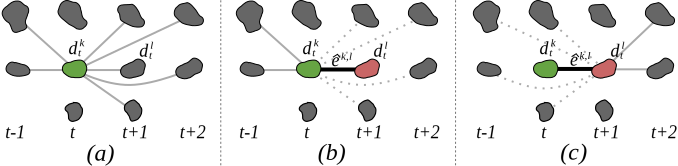
\includegraphics[width = 100mm] {images/greedytracking.pdf}\\ [-2.4ex]
       \end{tabular} 
    \caption{  {\footnotesize {\it Greedy  Tracking.}  {\em  (a)} The algorithm begins with each
        detection fully connected to all future and past detections
        within  a time  window  $W$.  Above, only  $d^k_t$'s edges  are
        shown. {\em  (b)} Each iteration,  the edge $\hat{e}^{k,l}$
        with   minimum  cost   $\hat{w}_e$  is  added  to $\mathcal{E}'$.   Edges  connecting
        $d^k_t$ to  future detections are  removed from $\mathcal{E}$.
        {\em  (c)} Edges  connecting  $d^l_t$ to  the past  are
        removed from $\mathcal{E}$.  The process is repeated until $\hat w_e > T$. }}
    \label{fig:greedytracking}
  
\end{figure}



\subsection{Evaluation: TODO}

%======================================================
\section{Neurites detection}\label{sec:neurite}
%======================================================
\subsection{Probabilistic Neuron Segmentation and Neurite Tree Extraction}
\label{sec:segmentation}
\vspace{-2mm}
Given an  image $I_t$  and the set  of somata  present in it  $S_t=\{s_t^1 \dots
s_t^m \}$,  our goal is  to associate  to each pixel  $u$ a label  $J_t(u)$ that
indicates to which soma it belongs.   The probability of $J_t(u)$ can be deduced
using Bayes' rule,
%\vspace{-1mm}
\begin{equation}
  \label{eq:bayes}
  P(J_t(u)=i|S_t,I_t) = \frac{P(S_t,I_t| J_t(u)=i)}{\sum_{\eta=1}^m P(S_t,I_t|J_t(u)=\eta)},
\end{equation}
\noindent  where we  have assumed  a uniform  distribution on  $P(J_t(u))$.  The
numerator  is modeled  as the  probability of the path $L$ that connects maximally 
the voxel $u$ to the soma $s_t^i$,
%% \begin{equation}
%%   \label{eq:shortestpath}
$  P(S_t,I_t| J_t(u)=i) = \max_{L:u\rightarrow  s_t^i}   \prod_{\{l_{r}\}
    \in L  } P(I_t(r)|l_{r}),$
%\end{equation}
where $l_{r}$ are indicator  variables for the locations forming the
path $L$. We chose this model  since an optimal maxima can be found
by minimizing its  negative likelihood using geodesic shortest  path \cite{Cohen96} and because
it produces connected components.

To optimize this function, we first compute geodesic distances from the tracked somata using the fast marching algorithm \cite{Sethian99,Cohen96}, applied on $P(I_t(v)|v)$, where $P(I_t(v)|v)$ represents the probability that a  neurite traverses a node $v$ and is
obtained  by  applying  a  sigmoid  function  to  the  output  of  the
tubularity filter  of~\cite{Frangi98}.  The parameters  of the sigmoid
function are  estimated using  maximum likelihood. 

Finally,  we define the set  of neurite pixels $U_n^t$  as those that connect  to any soma
with a higher probability than $\epsilon$.  We predict their labels as
the  ones  that  maximize   Eq.~\ref{eq:bayes}.   The  set  of  pixels
associated to neuron $X_t^i$ is the union of the neurites and the soma
associated  with $i$, $  U_i^t =  \{u \in  U_n^t |  J_t(u) =  i\} \cup
s_t^i$. To reduce  the neurite segmentation to a  tree, we skeletonize
the neuron and  define as root node the pixel  of the skeleton closest
to the centroid of the nucleus. We instantiate a Minimum Spanning Tree
from the  root and create a  neurite tree every time the  the spanning tree
exits the soma.

%----------------------------------------------------------------------------
\begin{figure}[!b]
  \begin{center}
       \begin{tabular}{@{\hspace{1mm}}c@{\hspace{1mm}}c@{\hspace{1mm}}c}
        \includegraphics[width = 0.32\textwidth] {images/SomataDetected.png} & \includegraphics[width = 0.32\textwidth] {images/SomataTracked.png} & \includegraphics[width = 0.32\textwidth] {images/LocalProb.png}\\ 
	\includegraphics[width = 0.32\textwidth] {images/GeodesicDistance.png} & \includegraphics[width = 0.32\textwidth] {images/Voronoi.png} & \includegraphics[width = 0.32\textwidth] {images/KeyPoints.png}\\ 
       \end{tabular} 
    \caption{ \footnotesize  TODO.}
    \label{fig:NeuritesDetection}
  \end{center}
\end{figure}
%----------------------------------------------------------------------------


\subsection{Evaluation: TODO}

%======================================================
\section{Neurite Tracking and Filopodia Detection}\label{sec:neurite}
%======================================================

Neurites are tracked by applying the algorithm described in Sec~\ref{sec:tracking} using
the centroids of the neurite trees instead of nucleus centroids, with the additional 
constraint that edges may only exist between neurites that emanate from the same soma.
Filopodia are detected by starting at each leaf node in a neurite and traversing the tree until a branch
point is reached. If the distance traversed is less than a threshold $T_f$, the traversed locations
are considered to be filopodia.


%======================================================
\section{Filopodia detection}\label{sec:filo}
%======================================================

%%======================================================================
%%% -*- mode: latex; mode: reftex; mode: flyspell; TeX-master: "top.tex"; -*-

We  present  a  fully  automatic  method to  track  and  quantify  the
morphodynamics of  differentiating neurons in  fluorescence time-lapse
microscopy  datasets.    While  previous  efforts   have  successfully
quantified the dynamics of organelles  such as the cell body, nucleus,
or chromosomes of  cultured cells, neurons have proved  to be uniquely
challenging  due to  their  highly deformable  neurites which  expand,
branch, and collapse.  Our  approach is capable of robustly detecting,
tracking, and segmenting all the  components of each neuron present in
the sequence including the nucleus, soma, neurites, and filopodia.  To
meet  the   demands  required  for   high-throughput  processing,  our
framework is designed to be extremely efficient, capable of processing
a single image in approximately two seconds on a conventional notebook
computer.   For  validation  of  our approach,  we  analyzed  neuronal
differentiation datasets in  which a set of genes  was perturbed using
RNA interference. Our analysis confirms previous quantitative findings
measured  from   static  images,  as  well   as  previous  qualitative
observations of  morphodynamic phenotypes that could  not be measured
on a large scale. Finally,  we present new observations about the 
behavior of  neurons made  possible by our quantitative  analysis, which
are not immediately obvious to a human observer.

%  whose
%measurements were not feasible on a large scale.  Finally, using our
%quantitative analysis we make

%our dynamic
%quantitative analysis allows us to  make new observations that are not
%visible to a human observer.


%% we  use it to  perform an siRNA  screen and
%% successfully reproduce the findings of~\cite{}, which was performed at
%% steady-state under less stressful conditions [OLVIER, HELP US SAY THIS
%%   MORE  ELOQUENTLY].   Finally, we  apply  our  approach  to make  new
%% observations   based  on  dynamic   quantitative  analysis   that  was
%% previously impossible.

%% While  previous efforts
%% have tracked the soma and nucleus,  our approach is the first to fully automatically track
%% and reconstruct the neurites as  they expand, branch and collapse, and
%% to dynamically detect fine filopodia structures.

%We present a method to analyze and extract statistics from large-scale
%video sequences  of in-vitro neurons.   Our system is able  to detect,
%track, segment  and reconstruct each individual neuron  present on the
%videos.   We show how  such system  can be  used to  find correlations
%between neuron behaviour and the proteins used to mutate them.

%high throughput automation

%confirms pre-existing findings

%yields new understandings about the dynamic morphologies

%efficient, tracks, segments, and tracks neurites


%%======================================================================
%
%%======================================================================
%%% -*- mode: latex; mode: reftex; mode: flyspell; TeX-master: "top.tex"; -*-


The  process  of forming  functional  connections  between neurons  is
complex  and   dynamic.   Time-lapse  microscopy   has  revealed  that
differentiating  neurons undergo  a large  range of  dynamic processes
including cell body motility, filopodial dynamics, and repeated cycles
of  neurite growth  and  retraction.  Of  critical  importance is  the
process  by which  axons and  dendrites are  formed in  which a neurite
ceases retracting, extends a   long  distance, and  forms
a connection. Such  dynamic events are  governed by a  complex protein
network that  coordinates   dynamic functions 
within the cytoskeleton, membrane, etc.

Powerful tools such as 
RNA interference  (RNAi)
technology,  fluorescent  protein   labeling,  image  processing,  and
automated high-throughput  microscopy have  opened the door  for large
scale  perturbation studies to help investigate such processes. RNAi  screens have  already led  to novel
insights   into  a  number   of  cellular   processes  such   as  cell
migration~\cite{Bakal07}  and endocytosis~\cite{Collinet10}.  However,
limitations  in  image  processing  have  restricted  most
investigations to static image analysis.

Knowledge  of dynamics is  essential if we are  to understand
complex  processes such  as neuron  morphogenesis.  However, designing
algorithms to quantify dynamic  behaviors is challenging, and
automatic methods  have appeared only  very recently. State-of-the-art
high-throughput techniques have successfully quantified morphodynamics
of  HeLA cancer  cells  in an  effort  to understand  the process  of
mitosis~\cite{Held10,Neumann10,Zhu05}.   However,  the morphology  and
dynamics of  these cell types  are relatively simple compared to neurons,
whose highly deformable  neurites  branch, expand,
retract, and collapse. 


In this paper, we  propose a  fully  automatic method  for  detecting, tracking,  and
segmenting {\em every component of the neuron} (nucleus,  soma, neurites, and filopodia), and quantifying  their dynamic behaviors in ways that were previously not possible. Our approach first  detects nuclei at each time step.  A greedy  tracking algorithm  associates detected nuclei belonging
belonging to the same neuron,  forming a list of detections corresponding  
to that neuron.  Using  the detected nuclei as seed  points, a region-growing
algorithm segments the neuron's soma.  The somata are used to
initialize a joint segmentation of the entire structure of all neurons
appearing in  a image using  a probabilistic method based  on shortest
path computations.   A  graph describing the  morphology of
the  neurites is extracted from  this segmentation.  Each neurite 
tree is tracked by association, and filopodia are detected
by analyzing the topology of the tracked neurites. Finally, 
a set of 156 {\em morphodynamic features} is extracted, quantifying
the behavior of the each neuron in the video.


As   demonstrated  in   Fig.~\ref{fig:video}, 
our  approach produces reliable  segmentations capable of capturing
complex  neuron  dynamics. To validate our approach, we analyzed a   
small-scale  siRNA screen  of 5  genes (3  siRNAs/gene). Our analysis
confirmed steady-state phenotypes obtained previously using 
MetaMorph\texttrademark~\cite{Pertz08}. We were also able to
quantify dynamic behaviors which had been previously observed, but never
measured~\cite{Pertz08}. Our  analysis also uncovered
new dynamic behaviors which are only apparant through dynamic analysis.

%While  our greedy tracking  and probabilistic  segmentation algorithms are  novel,  they are designed to be efficient and thus are relatively simple.  The  main contribution of this  paper is the  system as a whole,  which  is capable  of  high-throughput  processing of  videos, tracking individual  parts of  neurons, and quantifying  their dynamic behaviors in ways that were previously not possible.


%----------------------------------------------------------------------------
\begin{figure}[t]
       \begin{tabular}{@{\hspace{0mm}}c@{}|@{}c@{}}
        \includegraphics[width=45mm] {images/mv1_005.png}  &
        \includegraphics[width=45mm] {images/mv1_008.png} \\ [-.8ex]
        \hline \\ [-2.6ex]
        \includegraphics[width=45mm] {images/mv1_017.png}  &
        \includegraphics[width=45mm] {images/mv1_026.png} \\ [-.8ex]
        \hline \\ [-2.9ex]
       \end{tabular} 
       
      \begin{tabular}{@{\hspace{0mm}}c@{}c@{}c@{}c@{}}
        \includegraphics[width=22.5mm] {images/0_005.png} &
        \includegraphics[width=22.5mm] {images/0_008.png} & 
        \includegraphics[width=22.5mm] {images/0_017.png} & 
        \includegraphics[width=22.5mm] {images/0_026.png} \\ [-1ex]
        \includegraphics[width=22.5mm] {images/2_005.png} &
        \includegraphics[width=22.5mm] {images/2_008.png} & 
        \includegraphics[width=22.5mm] {images/2_017.png} & 
        \includegraphics[width=22.5mm] {images/2_026.png} \\ [-1ex]
        %\includegraphics[width=22.5mm] {images/3_005.png} &
        %\includegraphics[width=22.5mm] {images/3_008.png} & 
        %\includegraphics[width=22.5mm] {images/3_017.png} & 
        %\includegraphics[width=22.5mm] {images/3_026.png} \\ [-1ex]
        {\footnotesize $t = 50$ min} & 
        {\footnotesize $t = 80$ min} & 
        {\footnotesize $t = 170$ min} & 
        {\footnotesize $t = 260$ min} \\ [-1ex]
      \end{tabular}
    \vspace{-2mm}  
    \caption{ {\footnotesize {\it Neuron  Tracking Results.  } The top
        two rows  contain frames from an experiment  where MAP2K7 gene
        functions are inhibited.  For visibility we enhanced the image
        contrast.  Tracked neurons are marked by a unique color and id
        tag.   Nuclei  are denoted  by  filled  ellipsoids, somata  as
        contours,  and neurites  as trees.   Bottom rows  show details
        from  above: 1)  enhanced original  image 2)  tracked neurites
        marked with a different colors. Our  approach   performs  well  even  in  challenging
        situations where neurons appear in close proximity. Note: faintly  stained
        cells are ignored for robustness.}}
    \label{fig:video}
\vspace{-6mm}
\end{figure}
%----------------------------------------------------------------------------



%%======================================================================
%
%%======================================================================
%%\begin{results}
%%======================================================================
%
%%======================================================================
%\input{experimental-basel.tex}
%%======================================================================
%
%%======================================================================
%%!TEX root =  main.tex
%======================================================================
\subsection{Automated computer vision analysis of neurite ougrowth dynamics}
%======================================================================
To capture the dynamic neurite outgrowth trajectories of neurons in the native and perturbed state, we developed a computer vision pipeline that allowed to automatically segment and track the soma and neurites in each frame of the timelapse datasets. Our approach first detects nuclei and associated somata at each time step. The nucleus of each neuron is detected as a Maximally Stable Extremal Region (MSER)6 from the Cherry channel. [As shown in the supplementary note 3, this is more robust than adaptive thresholding.] Using the detected nuclei as seed points, a region-growing algorithm segments the neuron�s soma. Next, the implemented multi-objects tracking algorithm7 searches through the full set of nuclei and somata detections to extract the best K-shortest paths according to a similarity measure between two detections. The proposed similarity measure is derived from the Earth Mover�s Distance8 between the intensity histograms of the detected somata regions (in the supplementary note 3, we show that this distance provides a good tradeoff between efficiency and precision).  Neurons are detected and tracked at an accuracy of (TODO 95\%) (more than 2000 objects TODO); �Finally, the tracked somata are used to initialize a neurite segmentation and association algorithm based on shortest path computation and Voronoi tessellation. Comparison to manually annotated data demonstrates that �(URGENT TODO: crunch the numbers)�





\textcolor{red}{
Fethallah and Kevin can you please write a 10 line long, accessible paragraph that explains the segmentation procedure and the quantification of its efficiency in comparison with the manually annotated ground truth. We can add a supplementary note (Supplementary note 3) that describes the process in depth.
}
Can you please also sketch figure 2 that is dedicated to the segmentation process. This figure will show:
\begin{enumerate}
\item raw green and red images (it is the 1st figure in which we will show this). 
\item schematics of successive steps in the image segmentation.
\item A fully segmented time series of neurons as an example.
\item Some kind of efficiency evaluation in comparison with the manually annotated ground truth.
\end{enumerate}
Please then write another paragraph that explains the different static and dynamic features that are extracted.
\textcolor{red}{
Please sketch figure 3, which explains graphically how some static and dynamic features are extracted. You can represent some of the trajectories of one or two features over time. For this, you can use one of the presentation that Kevin once made. I would try to show a graph of a feature trajectory that is stochastic like the protrusion/retraction cycles of neurite outgrowth. This shows that we look at highly dynamic events, and thus illustrates the benefit of our approach. We can add a number of supplementary movies with different morphological features that are analyzed (soma, each new neurites). Please prepare also supplementary tables about the definition of features (supp tables 1 and 2). Then we also need a supplementary note that explain the format in which the morphodynamic history of each cell is explained.}

%%======================================================================
%
%%======================================================================
%\input{analysis-idiap.tex}
%%======================================================================

%======================================================================
%\end{results}
%======================================================================


%======================================================================
%\bibliographystyle{naturemag}
\bibliography{vision}
%======================================================================

%\begin{addendum}
% \item Put acknowledgements here.
% \item[Competing Interests] The authors declare that they have no
%competing financial interests.
% \item[Correspondence] Phone: +41 61 267 22 03; Fax: +41 61 267 35 66; E-mail : \texttt{olivier.pertz@unibas.ch}.
%\end{addendum}

\end{document}


















%======================================================================

%% Example Figure commented
%FFFFFFFFFFFFFFFFFFFFFFFFFFFFFFFFFFFFFFFFFFFFFFFFFFFFFFFFFFFFFFFFFFFFFF
%\begin{figure}
%\caption{Each figure legend should begin with a brief title for
%the whole figure and continue with a short description of each
%panel and the symbols used. For contributions with methods
%sections, legends should not contain any details of methods, or
%exceed 100 words (fewer than 500 words in total for the whole
%paper). In contributions without methods sections, legends should
%be fewer than 300 words (800 words or fewer in total for the whole
%paper).}
%\end{figure}
%FFFFFFFFFFFFFFFFFFFFFFFFFFFFFFFFFFFFFFFFFFFFFFFFFFFFFFFFFFFFFFFFFFFFFF

%Figures
%Figure 1. Global pipeline to analyze neurite outgrowth morphodynamic phenotypes. (olivier and Ludo)
%Figure 2. Computer vision segmentation of neuronal morphodynamics feature extraction.
%(Fethallah and Kevin)
%Figure 3.  Description of morphodynamic features.
%(Fethallah and Kevin)
%Figure 4. Morphodynamic phenotype feature selection
%(Riwal)
%try to make a  series of schemes that explain the different steps in feature selection,
%vector distance, assessment of interplate and siRNA induced noise.
%
%Figure 5.  Morphodynamic phenotype description.
%(Riwal, Olivier, Ludo)
% this will consist of a color-coded map of the different features extracted for each gene perturbation, we will then focus on more specific aspects of what we learned.
%
% 
%Supplementary Figures.
%
%Figure S1. Experimental controls lifeact-GFP/NLS-mCherry reporter and siRNA transfection.
%(a) Structure of the Lifeact-GFP IRES NLS-mCherry expression vector. (b) Effect of Lifeact-GFP expression on neurite outgrowth.
%(ludo and olivier)
%
%
%Figure S2. Feature selection on synthetic data produced by mixing videos from different known sources to test the ability of the algorithm to appropriately identify different morphodynamic signatures (Riwal)
%
%
%
%?
%
%Supplementary tables.
%
%Table S1. Definition of static features.
%Table S2. Definition of dynamic features.
%
%
%
%?
%Supplementary notes
%
%Supplementary note 1. Description of RNA interference experiments.
%
%Olivier and ludo
%
%Supplementary note 2. Description of microscope setup used for high content acquisition.
%Olivier and ludo
%
%
%Supplementary note 3. In depth description of computer vision segmentation and evaluation of the method by comparison with ground truth.
%
%Fethallah and Kevin
%
%
%Supplementary note 4. Description of html format in which the cell trajectories are described
%
%Fethallah and Kevin
%
%?
%Supplementary movies.
%
%Supplementary movie 1. Representative timelapse movie of N1E-115 cells expressing the GFP-lifeact-IRES-NLS-mcherry construct with the 10x PlanApo objective.
%
%Supplementary movie 2. Representative timelapse movie of N1E-115 cells expressing the GFP-lifeact-IRES-NLS-mcherry construct with the 20x PlanApo objective.
%
%Supplementary movie 3.
%
%
%
%
%
% 
%References
%
%1.	B. Snijder, R. Sacher, P. Ramo et al., Nature 461 (7263), 520 (2009).
%2.	C. Collinet, M. Stoter, C. R. Bradshaw et al., Nature 464 (7286), 243 (2010).
%3.	M. Held, M. H. Schmitz, B. Fischer et al., Nature methods 7 (9), 747 (2010).
%4.	D. Loerke, Q. le Duc, I. Blonk et al., Science signaling 5 (231), rs5 (2012).
%5.	J. Riedl, A. H. Crevenna, K. Kessenbrock et al., Nature methods 5 (7), 605 (2008).

